\documentclass[10pt,a4paper]{article}

\usepackage[margin=1.5cm]{geometry}
\usepackage[UKenglish]{babel}
\usepackage{enumitem}
\usepackage{fancyhdr}
\usepackage{graphicx}
\usepackage{multirow}
\usepackage[table]{xcolor}
\usepackage{float}

\definecolor{titleColor}{RGB}{138,201,242}
\pagestyle{fancy}
\lhead{T Davies, A Fahie, A Fairbairn, A Free, J Mansfield, R Tucker, M Walker}
\chead{}
\rhead{GPIG-C}
\cfoot{\vspace{-1cm} \thepage}

\setlist{nolistsep} % Reduces lots of white space around lists

\renewcommand{\headrulewidth}{0.4pt} % Add rules below header

\begin{document}

\title{\vspace{-1cm}GPIG-C Initial Report}
\author{Word count: \textbf{??} according to \textsl{detex \$FILE $\vert$ wc -w}}
\date{Friday, 25th October}
\maketitle
\thispagestyle{fancy} % Make sure header and footer appear on the front page

\section{Introduction}

\subsection{Single statement of need}
This project aims to deliver a tailorable Health and Usage Monitoring System
(HUMS), tailorable to multiple target domains. The target for the system is any
consumer needing to collect, store, analyse and report data from one or more
data input clients.

\subsection{Intended audience of this document}
The intended audience of this document are both the developers and the customer.
The document is structured in a manner which will interest all concerned
parties. Requirements will follow the introduction, followed by use cases, a
review of possible solutions and a risk register.

\section{Use cases}
\noindent \textbf{ID:} UC1\\
\textbf{Name:} Monitoring a system.\\
\textbf{Context:} The organisation has developed a system, for which they
require health and usage monitoring.\\
\textbf{Primary Actor:} The organisation's technical representative.\\
\textbf{Secondary Actors:} The health and usage monitoring system, the
organisation's system.\\
\textbf{Precondition:}  The organisation has a system that requires monitoring.
The organisation's system and environment must conform to the constraint
requirements detailed in this document. The end user has access to the
facilities required to install the HUMS. The end user has basic technical
computing knowledge.\\
\textbf{Trigger:} The end user sets up an account and attempts to integrate
their system.\\
\textbf{Main Success Scenario:} The end user successfully manages to integrate
their system with the HUMS.\\
\textbf{Main Success Postcondition:} The HUMS is successfully integrated with
the user's system, allowing data to be passed through the input and output
interfaces.\\
\textbf{Exception Scenarios:}
\begin{itemize}
\item The end user fails to integrate their system with the HUMS because their
system does not conform to the data input interface.
\item The end user fails to integrate their system with the HUMS because their
system does not conform to the output interface.
\item The end user chooses to abort the process.
\end{itemize}
\textbf{Exception Postcondition:} If the end user's system could not be
integrated with the HUMS, the user is provided with diagnostic information and
technical support needed to solve any problems. If the end user chose to quit
the process, they are presented with access to technical support.\\\\
\noindent \textbf{ID:} UC2\\
\textbf{Name:} Analysing collected data.\\
\textbf{Context:} The organisation wishes to define how their data should be
analysed.\\
\textbf{Primary Actor:} The end user.\\
\textbf{Secondary Actors:} The HUMS.\\
\textbf{Precondition:}
\begin{itemize}
\item The user has set up an account.
\item The organisation's sensor system and the HUMS have been successfully
integrated.
\end{itemize}
\textbf{Trigger:} The user decides how they want to analyse their data
abstractly.\\
\textbf{Main Success Scenario:}
\begin{itemize}
\item The user creates a concrete implementation of their abstract analysis
system and interfaces it with the HUMS, allowing them to analyse data as per
their definition.
\item We implement an analysis system on the user's behalf. The HUMS then
analyses data as as defined by the user.
\end{itemize}
\textbf{Main Success Postcondition:} User can analyse data stored in the HUMS.\\
\textbf{Exception Scenarios:} User's analysis system does not conform to the
analysis interface.\\
\textbf{Exception Postcondition:} HUMS can still collect and store data.\\\\
\noindent \textbf{ID:} UC3\\
\textbf{Name:} Reporting and notifications\\
\textbf{Context:} The organisation's sensor system, analysis system and the HUMS
have been successfully integrated, and they now wish to define how users should
be notified of events or receive reports.\\
\textbf{Primary Actor:} End user\\
\textbf{Secondary Actors:} The HUMS.\\
\textbf{Precondition:}
\begin{itemize}
\item The user has set up an account
\item The organisation's sensor system, analysis system and the HUMS have been
successfully integrated.
\end{itemize}
\textbf{Trigger:} The user decides on the format and communication method used
to keep them informed of the state of the system.\\
\textbf{Main Success Scenario:}
\begin{itemize}
\item The user implements a notification and reporting system with correctly
integrates with the HUMS to keep end users informed.
\item We implement a notification and reporting system on behalf of the
customer, allowing them to receive updates about the state of the system they
are monitoring.
\end{itemize}
\textbf{Main Success Postcondition:}
\begin{itemize}
\item The user is notified when the analysis system fires an event
\item The user can request reports
\end{itemize}
\textbf{Exception Scenarios:} User's notification and reporting system
implementation does not conform to the notification and reporting interface and
so cannot function correctly.\\
\textbf{Exception Postcondition:} HUMS can still collect, store and analyse
data.

\section{Requirements}
For this project, requirements have been divided into three categories,
functional, non-functional and constraint. The requirements have been
engineered such that each falls into one of those three categories, this
prevents them from becoming too complex. Each requirement has been
structured as simply and concisely as possible and been worded in such a way
as to avoid ambiguity. The requirements represent the problem to be solved
and serve as a contract between us, as the development team, and the
customer. All requirements have therefore been checked with the customer to
ensure the system described is the system they envisioned.\\
functional requirements detail what inputs, behaviour and outputs the system
must provide. The non-functional requirements specify the qualities of the
system as opposed to its behaviour. Constraint requirements are those that apply
to the entire system, including any constraints on the environment the system
can be used in and any timing constraints. In order to ensure all requirements
are verifiable, appropriate testing procedures have been included.

\subsection{Functional Requirements}
\subsubsection{Sensing Data}
\begin{table}[H]
\vspace{-0.5cm}
    \begin{tabular}{| p{1.1cm} | p{6cm} | p{9cm} | }
    	\hline
    	\cellcolor{titleColor}\textbf{ID}   & \cellcolor{titleColor}\textbf{Description}                                                              & \cellcolor{titleColor}\textbf{Verification}                                                                                                                                                                                                                                     \\ \hline
    	\textbf{FR.1} & Data input clients shall be able to push correctly structured data to the system. & Unit Testing 
	\begin{itemize} 
	\item Attempt to send correctly structured data to the system. Assert the data is correctly received.
	 \item Attempt to send incorrectly structured data to the system. Assert the data failed structure validation.
	 \end{itemize} \\ \hline
    	\textbf{FR.2} & The system shall allocate a timestamp to new data.                                & Unit Testing\begin{itemize} \item Assert data is timestamped.\item Assert there is a ��happens before�� relation between any pair of timestamps, such that timestamps reflect the order in which data arrives.\end{itemize}\\ \hline
	\end{tabular}
\end{table}
\subsubsection{Storing Data}
\begin{table}[H]
\vspace{-0.5cm}
    \begin{tabular}{| p{1.1cm} | p{6cm} | p{9cm}| }
        \hline
        \cellcolor{titleColor}\textbf{ID}    & \cellcolor{titleColor}\textbf{Description}                                                                                                                           & \cellcolor{titleColor}\textbf{Verification}                                                                                                                                                                                                                                                                    
        \\ \hline
        \textbf{FR.3}  & The system shall store correctly structured data.                                                                                              & Unit Testing\begin{itemize} \item Attempt to store correctly structured data in the system. Assert that the data can be retrieved.\item Attempt to store incorrectly structured data in the system. Assert that the data is rejected.\end{itemize}                                \\ \hline
        \textbf{FR.4}  & The system shall allow the consumer to define a low storage threshold.                                                                         & Black Box Testing\begin{itemize} \item Attempt to set a low storage threshold. Assert attempt is successful.\end{itemize}                                                                                                                                                           \\ \hline
        \textbf{FR.5}  & The system shall send a notification when the consumers defined low storage threshold is reached.                                              & Unit Testing\begin{itemize} \item Simulate reaching the low storage threshold. Assert that the method invoking a notification is called.\end{itemize}                                                                                                                               \\ \hline
        \textbf{FR.6}  & The system shall allow the consumer to set an expiry time on data.                                                                             & Grey Box Testing\begin{itemize} \item Attempt to set an expiry time on data. Add the data to the system. Assert the data has been stored with the expiry time.\end{itemize}                                                                                                         \\ \hline
        \textbf{FR.7}  & The system will delete data when its expiry time is reached.                                                                                   & Integration Testing\begin{itemize} \item Assert no stored data is older than its defined expiry time.\end{itemize}                                                                                                                                                                  \\ \hline
        \textbf{FR.8}  & The system must store no more data records than the consumers defined storage quota.                                                           & Integration Testing\begin{itemize} \item Assert the maximum number of data records held by the consumer is less than or equal to their defined quota.\end{itemize}                                                                                                                  \\ \hline
        \textbf{FR.9}  & The system shall allow the user to define that, upon reaching their defined data storage quota, new data is no longer added.                   & Unit Testing\begin{itemize} \item Simulate reaching the an arbitrary storage quota. Attempt to send more data to the system. Assert the send failed due to insufficient storage.\end{itemize}                                                                                       \\ \hline
    	\textbf{FR.10} & The system shall allow the user to define that, upon reaching their defined data storage limit, old data is deleted to make room for new data. & Unit Testing\begin{itemize} \item Simulate reaching the an arbitrary storage quota. Attempt to send more data to the system. Assert the send succeeded and the new data has been added to storage. Assert that the previous oldest record in storage has been deleted.\end{itemize} \\ \hline
	\end{tabular}
\end{table}
\subsubsection{Analysing Data}
\begin{table}[H]
\vspace{-0.5cm}
    \begin{tabular}{| p{1.1cm} | p{6cm} | p{9cm} |}
        \hline
        \cellcolor{titleColor}\textbf{ID}    & \cellcolor{titleColor}\textbf{Description}                                                                                      & \cellcolor{titleColor}\textbf{Verification}                                                                                                                                     \\ \hline
        \textbf{FR.11} & The system shall allow the consumer to specify what patterns of data will produce events.                 & Black Box Testing\begin{itemize} \item Assert that a specification of a valid pattern within a valid set of data succeeds.\end{itemize}              \\ \hline
        \textbf{FR.12} & Events shall be triggered in response to new data that matches a pattern that the consumer has specified. & Unit Testing\begin{itemize} \item Send the system a pattern of data which is known to constitute an event. Assert an event is produced.\end{itemize} \\ \hline
    \end{tabular}
\end{table}
\subsubsection{Reporting Events}
\begin{table}
    \begin{tabular}{| p{1.5cm}| p{6cm}| p{9cm}|}
        \hline
        \cellcolor{titleColor}\textbf{ID}    & \cellcolor{titleColor}\textbf{Description}                                                                                                                                              & \cellcolor{titleColor}\textbf{Verification}                                                                                                                                                                                                                                                                                                                                      \\ \hline
        \textbf{FR.13} & The system shall dispatch a notification to the data output client after an event has occurred.                                                                  & Unit Testing\begin{itemize}\item Simulate an event occurring. Assert that the method producing a notification is invoked.\end{itemize}                                                                                                                                                                                                               \\ \hline
        \textbf{FR.14} & The consumer shall be able to assign types to events.                                                                                                            & Black Box Testing\begin{itemize}\item Attempt to assign a valid type to a valid event. Assert the attempt is successful.\end{itemize}                                                                                                                                                                                                                \\ \hline
        \textbf{FR.15} & The consumer shall be able to assign a cool down period for each type of event.                                                                                  & Grey Box Testing\begin{itemize}\item Simulate the customer setting a cool down period. Assert the attempt is successful.\end{itemize}                                                                                                                                                                                                                \\ \hline
        \textbf{FR.16} & After the sending of a notification for an event of a particular type, no more notifications for an event of that type will be sent during the cool down period. & Black Box Testing\begin{itemize}\item Simulate the customer setting a cool down period and then multiple events of the same type being triggered. Assert only one notification during each cool down period is sent.\end{itemize}                                                                                                                    \\ \hline
        \textbf{FR.17} & The system must allow data output clients to pull reports from the system.                                                                                       & Unit Testing\begin{itemize}\item Attempt to pull a data report from the system. Assert attempt is successful. Assert received data is correct.\end{itemize}                                                                                                                                                                                          \\ \hline
        \textbf{FR.18} & The system shall allow the consumer to set which data output clients can pull reports.                                                                           & Unit Testing\begin{itemize}\item Attempt to set which output clients can pull reports.\item Attempt to send a report to an output client who is allowed to receive them and verify that it succeeds.\item Attempt to send a report to an output client who is not allowed to receive them and verify that it fails.\end{itemize}                 \\ \hline
    	\textbf{FR.19} & The system shall allow the consumer to set which output clients can be sent notifications.                                                                       & Unit Testing\begin{itemize}\item Attempt to set which output clients can be sent notifications.\item Attempt to send a notification to an output client who is allowed to receive them and verify that it succeeds.\item Attempt to send a notification to and output client who is not allowed to receive them and verify that it fails.\end{itemize} \\ \hline
	\end{tabular}
\end{table}


\subsection{Non-functional requirements}

\subsubsection{Maintainability}
\begin{table}[h!]
\vspace{-0.5cm}
    \begin{tabular}{|p{1.5cm}|p{6.0cm}|p{9.0cm}|}
    \hline
    \cellcolor{titleColor}\textbf{ID} & \cellcolor{titleColor}\textbf{Description} & \cellcolor{titleColor}\textbf{Verification} \\ \hline
    \textbf{NFR.1} & The system shall be able to receive hardware changes without loss of previously stored data. & Recovery Testing\begin{itemize}\item Take a snapshot of a live system. Change a piece of hardware on the system and then check that, after the change, the data is still consistent with the snapshot.\end{itemize} \\ \hline
    \end{tabular}
\end{table}

\subsubsection{Accessibility}
\begin{table}[h!]
\vspace{-0.5cm}
    \begin{tabular}{|p{1.5cm}|p{6.0cm}|p{9.0cm}|}
    \hline
    \cellcolor{titleColor}\textbf{ID} & \cellcolor{titleColor}\textbf{Description} & \cellcolor{titleColor}\textbf{Verification} \\ \hline
    \textbf{NFR.2} & Users shall be provided with documentation detailing how to use the system. & Acceptance Testing\begin{itemize}\item We will require a receipt verifying the availability and standard of the documentation when allowing the user access to the system documentation.\end{itemize} \\ \hline
    \textbf{NFR.3} & The system, when running externally on servers, must be accessible to end users who are in multiple geographic locations. & Black Box Testing\begin{itemize}\item Assert the networked system can be accessed from multiple geographic locations.\end{itemize} \\ \hline
    \end{tabular}
\end{table}

\subsubsection{Security}
\begin{table}[h!]
\vspace{-0.5cm}
    \begin{tabular}{|p{1.5cm}|p{6.0cm}|p{9.0cm}|}
    \hline
    \cellcolor{titleColor}\textbf{ID} & \cellcolor{titleColor}\textbf{Description} & \cellcolor{titleColor}\textbf{Verification} \\ \hline
    \textbf{NFR.4} & The system shall only accept data from an input client providing valid credentials. & Unit testing\begin{itemize}\item Check that system both rejects unauthorised data and successfully accepts data from a source with valid credentials.\end{itemize} \\ \hline
    \textbf{NFR.5} & The system shall store data according to the relevant industry security standards. & Acceptance testing\begin{itemize}\item Have system externally verified against relevant standard setting body guidelines.\end{itemize} \\ \hline
    \end{tabular}
\end{table}

\subsubsection{Testability}
\begin{table}[h!]
\vspace{-0.5cm}
    \begin{tabular}{|p{1.5cm}|p{6.0cm}|p{9.0cm}|}
    \hline
    \cellcolor{titleColor}\textbf{ID} & \cellcolor{titleColor}\textbf{Description} & \cellcolor{titleColor}\textbf{Verification} \\ \hline
    \textbf{NFR.6} & The system shall be tested to ensure all requirements are met before deployment. & System Testing\begin{itemize}\item Make sure all tests of other requirements have passed.\end{itemize} \\ \hline
    \textbf{NFR.7} & The customer will complete acceptance testing before the system is deployed. & Acceptance Testing\begin{itemize}\item The customer will be required to sign off the project upon passing acceptance testing.\end{itemize} \\ \hline
    \end{tabular}
\end{table}

\subsubsection{Scalability}
\begin{table}[h!]
\vspace{-0.5cm}
    \begin{tabular}{|p{1.5cm}|p{6.0cm}|p{9.0cm}|}
    \hline
    \cellcolor{titleColor}\textbf{ID} & \cellcolor{titleColor}\textbf{Description} & \cellcolor{titleColor}\textbf{Verification} \\ \hline
    \textbf{NFR.8} & The system must be able to support at least 5 output clients per HUMS instance. & Black box testing\begin{itemize}\item Set up a HUMS instance and add 5 output clients and verify each can be sent a report.\end{itemize} \\ \hline
    \textbf{NFR.9} & The system must cope with up to 2000 data input requests per second per HUMS instance. & Grey Box Testing\begin{itemize}\item Set up a HUMS instance and send it 2000 data valid input requests per second and verify that all data is stored in the system.\end{itemize} \\ \hline
    \end{tabular}
\end{table}

\subsubsection{Reliability}
\begin{table}[h!]
\vspace{-0.5cm}
    \begin{tabular}{|p{1.5cm}|p{6.0cm}|p{9.0cm}|}
    \hline
    \cellcolor{titleColor}\textbf{ID} & \cellcolor{titleColor}\textbf{Description} & \cellcolor{titleColor}\textbf{Verification} \\ \hline
    \textbf{NFR.10} & The system must be available for no less than 99.9\% of each month. & Alpha testing\begin{itemize}\item Allow the system to be used as it would be in the real world for one month and check that it is available for the required amount of time.\end{itemize} \\ \hline
    \textbf{NFR.11} & Data must be backed up within 24 hours of having been made available to the system. & Integration testing\begin{itemize}\item Run the system for over 24 hours and verify that any data older than 24 hours exists in the back ups.\end{itemize}White Box Testing\begin{itemize}\item Verify there is a method in place to automatically back up data before it being 24 hours since having been made available to the system.\end{itemize} \\ \hline
    \textbf{NFR.12} & Timestamps applied by the system must be accurate to within 5ms of UTC. & Grey Box Testing\begin{itemize}\item Send the system the maximum number of supported data input requests per second and check that all timestamps are to within the given accuracy.\end{itemize} \\ \hline
    \textbf{NFR.13} & The system shall dispatch notifications within 5ms of the event being triggered. & Unit Testing\begin{itemize}\item Simulate an event. Assert that the notification is dispatched within the time period specified.\end{itemize} \\ \hline
    \end{tabular}
\end{table}


\subsection{Constraint Requirements}
\subsubsection{System Environment}
\begin{table}[h!]
	\begin{tabular}{| p{1.5cm} | p{15cm} |}
		\hline
		\textbf{ID}		&	\textbf{Description}	\\	\hline
		\textbf{CR.1}      &       A valid data schema defining the form of data that will be entered into the system will be provided.         \\ \hline
		\textbf{CR.2}      &       A valid data schema defining the form of data that will be stored the system will be provided.         \\ \hline
		\textbf{CR.3}      &       The system will be presented with valid credentials by the consumer’s data input clients.         \\ \hline
		\textbf{CR.4}      &       Valid output clients for the system will be specified by the consumer.         \\ \hline
		\textbf{CR.5}      &       The hardware that the system runs on will support the runtime of our software solution.         \\ \hline
		\textbf{CR.6}      &       The system will have access to the network to which the data sources are connected.         \\ \hline
	\end{tabular}
\end{table}

\subsubsection{Time}
\begin{table}[h!]
	\begin{tabular}{| p{1.5cm} | p{15cm} |}
		\hline
		\textbf{ID}		&	\textbf{Description}	\\	\hline
		\textbf{CR.7}      &       The customer will receive an initial project plan detailing the project requirements no later than October 25th 2013.         \\ \hline
		\textbf{CR.8}      &       The customer will receive an interim report detailing project progress no later February 14th 2014.         \\ \hline
		\textbf{CR.9}      &       The customer will receive a final report detailing the proposed system no later than May 28th 2014.         \\ \hline
		\textbf{CR.10}      &       The customer will be presented with a system prototype on May 30th 2014.         \\ \hline
	\end{tabular}
\end{table}

\subsubsection{Development}
\begin{table}[h!]
	\begin{tabular}{| p{1.5cm} | p{15cm} |}
		\hline
		\textbf{ID}		&	\textbf{Description}	\\	\hline
		\textbf{CR.11}      &       The development team will be comprised of seven software engineers.         \\ \hline
		\textbf{CR.12}      &       Any requirement changes outside of this document will be negotiated separately.         \\ \hline
	\end{tabular}
\end{table}


\section{Possible solutions}
When examining possible HUMS solutions, we inspected sensing, storing, analysing
and reporting data separately. This was done so that the best choice for each
could be individually selected, ensuring every sector of the system performs to
the highest possible standard. 
\\ \\
When examining how the HUMS should sense new data we identified three distinct
options:
\begin{enumerate}
\item Data input clients are directly linked to the system, with data being
pushed or polled depending on client support. This requires the system to
implement custom data specifications which is likely to become infeasible as the
system expands across domains.
\item Unmanaged data input clients which store data elsewhere. The HUMS polls
for data at the customers request. This option is slower and more inefficient
than having data pushed to the system, however may integrate better with
existing data input clients, reducing workload for the consumer.
\item Provide an input API which data input clients wishing to push data to the
system must implement. This option is the most flexible, allowing the system to
be integrated with any consumer system, in any domain. It does potentially mean
more work for the consumer in migrating existing systems to use the provided
API. \\
\end{enumerate}
When considering options for how to store data there are two core methods, an
SQL or NoSQL database. Using an SQL database would provide the consumer with
guaranteed atomicity, consistency, isolation and durability (ACID), thereby
offering reliability over throughput. Migration for the consumer may be easier
when using an SQL database, as SQL has been popular among enterprises for a long
time. SQL however does not easily scale horizontally, making it difficult to
expand one system across a large number of consumers. NoSQL solves the problem
of scalability at the expense of ACID compliance. Polyglot persistence offers a
solution to all of the problems identified when choosing between SQL and NoSQL,
by allowing the use of both. When using polyglot persistence the type and
structure of every type of data must be examined to determine which datastore is
most suitable, whether SQL or NoSQL.
\\ \\
When designing the data analysis segment of the system there are three feasible
implementations:
\begin{enumerate}
\item A plugin API, which allows users to implement their own analysis rules.
The system would provide multiple layers of abstraction, allowing the consumer
to take control of analysis at the level they see fit. For example, using a low
level API may be faster and allow greater customisation, but a web API is more
generic and easier for the consumer to implement.
\item Providing a rules engine for analysis, allowing the consumer to specify
and integrate their analysis requirements at a high level. This option would be
useful from the consumers perspective, abstracting from any low level
interfacing with the HUMS, but increasing the workload for our team.
\item Create customised single-purpose tools for each domain. This would be
massively inefficient from a development perspective, as well as costly and
inflexible. However the consumer may prefer to have a system completely designed
around their needs. \\
\end{enumerate}
For the reporting segment of the HUMS there are again multiple options.
Consumers may wish to pull reports from the system at specified times, or want
the system to notify another system or end user when an event has occurred. When
considering the consumer requesting a data report, we could provide them with a
single output format such as PDF or XML, however this is not very flexible and
is unlikely to provide the required functionality for all consumers. Another
option is to allow the user to directly access the HUMS datastore, however this
would leave the system open to data inconsistencies and expose implementation
detail to the consumer. A more flexible solution would be to provide a generic
reporting API to which plugins can be added. Each plugin would add a different
report format, allowing the consumer to choose which they wish to use in each
situation. This solution would be highly flexible, with new plugins being added
as the HUMS extends across domains.
\\ \\
When pushing notifications to another system or user, the HUMS could send events
encoded with a standard data interchange format, for example JSON or XML. This
would allow them to process the output themselves. The HUMS could also provide a
set of plugins allowing the consumer to choose what type of notification is
triggered when an event of a specific type occurs. For example, the system could
send an email for passive events but a mobile push notification or text message
for an event that requires urgent action. Allowing a variety of notification
channels provides a much more tailorable and maintainable product, but it
requires more development time and effort.

\subsection{Proposed solution}
Our proposed solution uses the concept of a client-server architecture, where
the client is the consumer?s system, sensing the data, and the server is the
system processing the data. These could exist within the same package or on the
same device, but they could also be geographically-distant machines connected
across the internet. The solution brings together the best elements from our
possible solutions for each section of the system, utilising a plugin
architecture for several components.
\\ \\
We will provide an input API for data input clients to push new data to the
system, accepting any correctly formatted sensor data sent on the correct
network (\textbf{DD.1}). Achieving correctly formatted data may require changes
to the consumers system, or using middleware. This approach makes our system
flexible, supporting a wide range of data input clients, meaning in future the
solution could easily extend across domains.
\\ \\
For data storage, the only applicable solution in this scenario is a database
(\textbf{DD.2}). Using polyglot persistence gives us the option of choosing a
database technology most suited to the consumer?s needs, which we will determine
during development. To make our choice we will look at all the relevant
technologies available and evaluate strengths and weaknesses in relation to
other design decisions for the data being stored, and how it will be accessed.
\\ \\
The data analysis part of the system will provide plugins offering analysis
tools, as well as an API for consumers to extend and create their own
specialised analysis rules (\textbf{DD.4}). Offering an API makes the system
more tailorable to different consumers and domains, as generic analysis tools
could not hope to meet every consumers needs by itself. Since some customers may
not want to take on the task of creating a whole analysis system themselves, we
will offer domain-specific plugins to simplify the process. This might include
graphical tools or other user-friendly features. The range of plugins offered
can be expanded as the system expands into more domains.
\\ \\
The system will include various output features for generating reports
(\textbf{DD.5}) and providing notifications (\textbf{DD.6}). For reports, we
will allow the consumer to customise the types of reports created. They will be
able to request reports in a variety of formats, including human-friendly
formats, e.g. PDF, and common data interchange formats. Consumers can use these
data formats as a data API to build their own reports or for any other purpose.
This will allow the consumer flexibility to produce what they want, whilst also
offering them easy to use built-in tools.
\\ \\
Our system will provide plugins to support various types of notification that
can be triggered based upon customisable events. Notifications will include 
emails, alongside more generic notifications formatted in standard formats such
as XML, just as with reports. The generic notifications could then be processed
further by the consumer, allowing them to tailor how notifications are used and
delivered.
\\ \\
The system will also provide an administration centre (\textbf{DD.3}) that lets
the consumer configure any customisable system settings including, setting up
events that trigger notifications and defining data schemas. This tool will be
offered through an intuitive web based interface which is only accessible by the
authorised consumer.
\\ \\
For the prototype we hope to demonstrate at the end of the project, we plan to
implement most of the solution described above. The core of the system,
including sensing, storing, analysing and reporting data, will be functional,
as will some of the basic components built utilising the plugin architecture.
Some additional simple components may be required when demonstrating, such as a
tool to simulate data being input to the system. 

\subsubsection{Design Decision}
\vspace{-0.5cm}
\begin{longtable}[H]{ | p{2cm} | p{3.5cm} | p{11cm} | }
		\hline
			\cellcolor{titleColor}\textbf{Design Decision ID}&	\cellcolor{titleColor}\textbf{Requirements Fulfilled}&	\cellcolor{titleColor}\textbf{Description}	\\ \hline
			\textbf{DD.1}&	FR.1, FR.2&	Provide an input API which data input clients wishing to push data to the system must conform to.	\\ \hline
			\textbf{DD.2}&	FR.7, FR.8&	Use a database to store data.	\\ \hline
			\textbf{DD.3}&	FR.4, FR.5, FR.6 FR.9, FR.10, FR.14, FR.15, FR.18, FR.19&	The system will provide an admin centre which allows the consumer to define data schemas and any configurable system settings.	\\ \hline
			\textbf{DD.4}&	FR.11&	The system will provide an analysis API, which the consumer can choose to implement, it will also provide a set of plugins conforming to this API which perform commonly used analysis functions.	\\ \hline
			\textbf{DD.5}&	FR.17&	The system will provide a set of plugins which allow the consumer to pull reports from the system in a variety of common formats, including high level formats such as PDF and low level formats such as XML.	\\ \hline
			\textbf{DD.6}&	FR.13, FR.13, FR.16&	The system will provide a set of plugins which push notifications of different formats to end users or data output clients.	\\ \hline
\end{longtable}


\begin{figure}[hptb]
  \centering
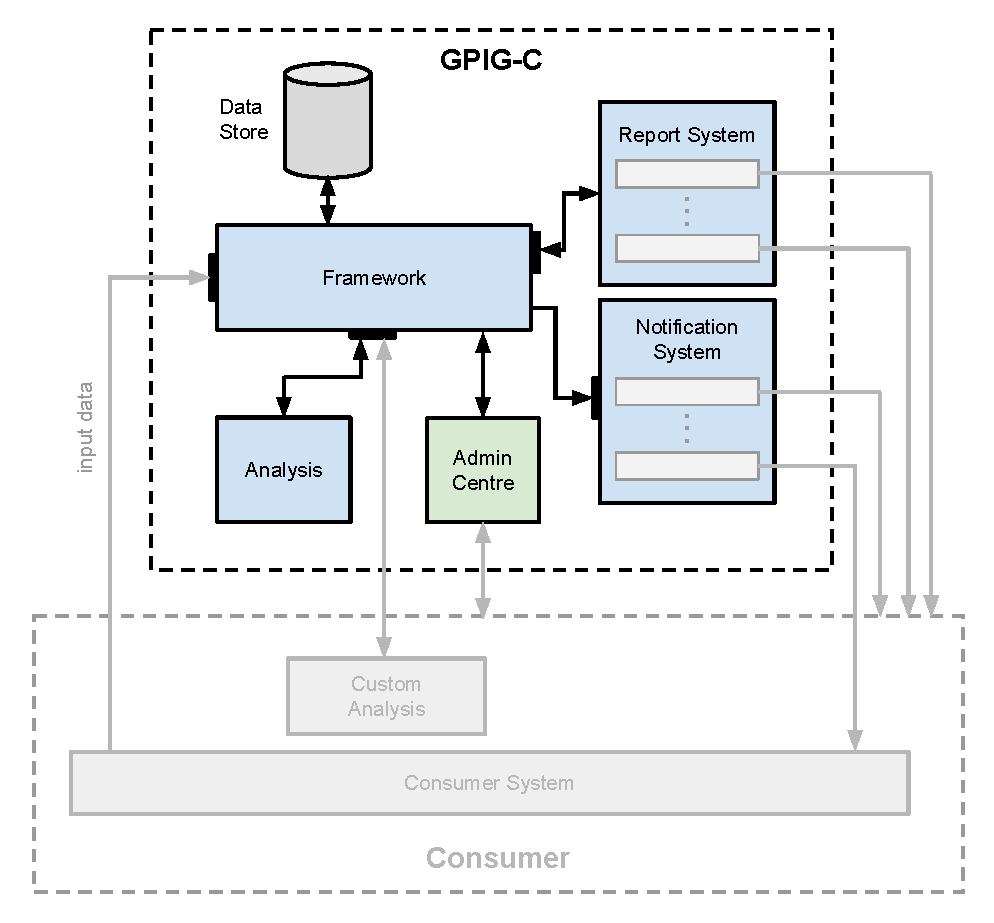
\includegraphics[width=0.75\textwidth]{system-architecture.pdf}
  \caption{System diagram}
\end{figure}

\section{Team organisation}

\subsection{Team members}
A list of team members is provided below, accompanied by a list of roles and
assignments relevant for the course of the project. The responsibilities have
been divided in a such a way that effort for all team members is equal and
fairly distributed. Assignees have been given roles which, where possible,
utilise their identified skills, and minimise exposure to established
weaknesses. \\
\\
\begin{tabular}{  p{4cm}  p{4cm}  p{4cm} p{4cm}  }
\textbf{AJF}-Adam Fahie            &         \textbf{AIF}-Andrew Fairbairn    &     \textbf{TF}-Anthony Free          &        \textbf{TD}-Tom Davies \\
\textbf{JM}-Joseph Mansfield     &        \textbf{RT}-Rosy Tucker           &          \textbf{MW}-Michael Walker \\
\end{tabular}

\subsection{Roles}
\subsubsection{Administrator Roles} 
\begin{table}[H]
\vspace{-0.5cm}
\begin{tabular}{ | p{3.5cm} | p{8.5cm} | p{4.5cm} |}
\hline
\cellcolor{titleColor}\textbf{Role}	        &   \cellcolor{titleColor}\textbf{Description}                                                                   & \cellcolor{titleColor}\textbf{Assignees}                         \\ \hline
Point of Contact         &   Buffer between customer and team.                                        & RT                                                 \\ \hline
Team Coordinator      &   Manage team communication and organise meetings.            & JM           				         \\ \hline
Minutes Secretary     &   Take minutes during meetings.                                                & AJF,AIF,TF,TD,JM,RT,MW             \\ \hline

\end{tabular}
\end{table}

\subsubsection{Technical Roles}
\begin{longtable}[H]{ | p{3.5cm} | p{8.5cm} | p{4.5cm} |}
\hline
\cellcolor{titleColor}\textbf{Role}	       		&   \cellcolor{titleColor}\textbf{Description}                                                                   											& \cellcolor{titleColor}\textbf{Assignees}                  \\ \hline
Editors         			&   Review and format draft documentation.                                        											& JM,TD,RT                               \\ \hline
Software Architect      	&   Responsible for ensuring requirements are met, and software is consistent.         								& AJF         			 	\\ \hline
Requirements Analysis     &   Identification of customer needs and requirements.                                              								& RT,AJF,JM,TD,AIF 		\\ \hline
Developer         		&   Developing software to agreed standards.                                      		 								&  AJF,AIF,TF,TD,JM,RT,MW     \\ \hline
UX/UI Designer     		&   Accessibility, UI/UX and user stories.							                								& JM,RT,AIF           			 \\ \hline
Security     			&   Advising on relevant security standards and protocols.                                           								& TF,MW				   	 \\ \hline
Penetration Tester       	&   Test HUMS for exploits and security weaknesses.                           	                 							& AJF,TF,AIF,TD,MW              	\\ \hline
Software Tester     		&   Creating or assisting in the creation of tests.          													& AJF,AIF,TF,TD,JM,RT,MW  	 \\ \hline
Risk Manager     		&   Enhancing chance of a successful delivery.                                               									& RT.TD				   	 \\ \hline
Database Admin		&   Design of database strategies and schemas.                            		                 							& AJF,AIF,MW                           	 \\ \hline
Legal    				&   Avoiding copyright license and patent violations.          					       								& JM           				 \\ \hline
Quality Assurance             &   Ensure cohesion between system modules, analysing system performance and enforce code quality standards.  		& JM,TD				    	\\ \hline
Product Owner        		&   Representing the views of the customer.                                       										 	& RT                                        	\\ \hline
Scrum Master      		&   Ensuring Scrum process is followed by all team members, and ensuring good inter-team communication.            		& RT           				\\ \hline
\end{longtable}

\subsection{Time and Task Management}

\section{Development plan}

\subsection{Software engineering methodology}
When developing the HUMS system, we chose to take an agile approach to
development and team management. Our implementation will follow a plugin
architecture, with one central codebase providing the core functionality and
plugins which provide domain tailorability. If a non-agile approach was to be
taken, a plugin architecture would be infeasible as those methodologies require
all requirements and documentation to be completed before development commences.
For example, the V-Model and waterfall model are linear processes, where
requirements are only discussed and designed before implementation commences.
This linearity gives no support for changes in requirements during the later
phases. Given the time constraints and the need for the system to be able to
evolve into various domains, these linear development methodologies are
impractical. \\
Agile software development, however, allows the project to split into smaller
sub-projects called `iterations' \cite{hazzan2008agile}. Each iteration allows
for a different section of the project to be planned, documented, developed and
tested. It also allows for the development team to be split into smaller
sub-teams working simultaneously on different areas on the project. At the end
of each iteration project priorities can be re-evaluated and the team structure
altered. 
\cite{hazzan2008agile} identifies three key perspectives of software
development: human, organisational and technological. The scrum methodology
harnesses two of those perspectives, providing a platform for both team and
project organisation. Unfortunately scrum does not provide a clear approach to
development from a technological perspective, providing no clear guidelines on
how code should be created or structured. However, the test driven approach does
provide a clear method of developing software from a technological perspective.
This encourages the development of unit and acceptance tests before the
development of code, the code itself is then written to make the tests pass.
Using both methodologies side by side appears to be the best approach for this
project, allowing for a well managed and organised team to produce well
structured and reliable code. Feature driven development could be used in place
of test driven and would provide a good platform for plugin generation, allowing
each plugin to be designed and implemented independently. However, it conflicts
with the project organisation aspects of the scrum methodology, meaning they
could not be used together without creating confusion. Since the scrum method
provides more guidance for managing team structure and monitoring project
progress, feature driven development was discounted in favour of scrum.

\subsection{Schedule}


\section{Risk register}
\begin{longtable}[H]{| p{0.6cm} | p{2cm} | p{0.3cm} | p{2.6cm} | p{8.1cm} | p{0.7cm} |}
    \hline
    \cellcolor{titleColor}\textbf{Risk ID}   & \cellcolor{titleColor}\textbf{Risk}                                             &\cellcolor{titleColor}\textbf{LS}        & \cellcolor{titleColor}\textbf{Classification and Possible Impact}                                 & \cellcolor{titleColor}\textbf{Mitigation and Contingency} & \cellcolor{titleColor}\textbf{IS} \\ \hline                                                                                                                                                                                                                                                                                                                                                                                                                                                                                                                                
    \textbf{R.1}   & Short term loss of team members                  & 6       & \textit{Moderate}
\newline Deadline failure                                        
      &  The team can then reactively reallocate the team member's work across remaining team members. To aid with this, the team must proactively ensure that no work relating to the project is outside of team version control. Use of the scrum methodology proactively aids work reallocation, ensuring team members are aware of all assigned work. 
      & 18    \\ \hline
    \textbf{R.2}    & Long term loss of team members                   & 2 & \textit{Catastrophic}
\newline Deadline failure and low standard of deliverables 
    & If a team member is unavailable for an extended period, the team will react by notifying the customer and possible extending deadlines. The proactive procedures mentioned in \textbf{R.1} will also be followed to reduce the impact of this scenario.                                                                                                                                                                                                                                                                                            
    & 10    \\ \hline
    \textbf{R.3}     & Short or long term loss of resources             & 2 & \textit{Catastrophic}
\newline Deadline failure and loss of code base              
    & Proactive use of a source code repository, meaning code-base and history is decentralised. If the repository is lost, the data can be retrieved from the local repository copies and university backups.                                                                                                                                                                                                                                                                                                        
    & 10    \\ \hline
    \textbf{R.4}     & Team member under-performance                    & 3         & \textit{Major}
\newline Deadline failure and low standard  of deliverables            
    & Project plan must be feasible. The skills of the team as a whole, and individual team members must be proactively established early on and taken into account when assigning roles.                                                                                                                                                                                                                                                                                                                                                              
    & 12    \\ \hline
    \textbf{R.5}    & Mis-interpretation of requirements                & 3        & \textit{Major}
\newline Deliverables that are not valid                                        & 
    Requirements, design and implementation strategy must be proactively verified with the customer, this process is iterative, stopping when both customer and developers are content. Any changes to those requirements must result in re-negotiated deadlines.                                                                                                                                                                                                                                                                                    
    & 12    \\ \hline
    \textbf{R.6}    & Slow response to customer queries                & 3        & \textit{Major}
\newline Deadline failure and  low standard of deliverables         
    & Customer has assured a two working day response where possible. Further mitigation can be achieved by proactively communicating issues well in advance of deadlines.                                                                                                                                                                                                                                                                                                                                                                            
    & 12    \\ \hline
    \textbf{R.7}     & Failure to produce required system functionality & 2 & \textit{Catastrophic}
\newline Wasted time and loss of marks                        
    & Customer verification of requirements can counteract this risk. System testing, to ensure all agreed upon requirements are met, will also reduce this risk.                                                                                                                                                                                                                                                                                                                                                                                      
    & 10    \\ \hline
    \textbf{R.8}     & Missing internal team deadlines                  & 5            & \textit{Moderate}
\newline Project falls behind due to missing dependencies                     
    & Perform critical path analysis to identify tasks which will take the longest time and which are a prerequisite to others. A greater team effort can then be assigned to these areas if it seems likely to miss a deadline or halt progress elsewhere.                                           
    & 15    \\ \hline
\end{longtable}

\begin{longtable}[H]{c c l | c | c | c | c | c | }
		\cline{4-8}
		& & & \multicolumn{5}{ c| }{Impact Score (Least$\rightarrow$Most)} \\ \cline{4-8}
		& & & 1 & 2 & 3 & 4 & 5 \\ \cline{4-8}
		& & & Negligible& Minor & Moderate& Major & Catastrophic \\ \cline{1-8}
		\multicolumn{1}{ |c }{\multirow{7}{*}{Likelihood Score}} & \multicolumn{1}{ |c| }{7} & Certain & 7 & 14 & 21 & 28 & 35 \\ \cline{2-8}
		\multicolumn{1}{ |c }{} & \multicolumn{1}{ |c| }{6} & Almost certain & 6 & 12 & 18 & 24 & 30 \\ \cline{2-8}
		\multicolumn{1}{ |c }{} & \multicolumn{1}{ |c| }{5} & Probable& 5 & 10 & 15 & 20 & 25 \\ \cline{2-8}
		\multicolumn{1}{ |c }{} & \multicolumn{1}{ |c| }{4} & Chances about even & 4 & 8 & 12 & 16 & 20 \\ \cline{2-8}
		\multicolumn{1}{ |c }{} & \multicolumn{1}{ |c| }{3} & Probably not & 3 & 6 & 9 & 12 & 15 \\ \cline{2-8}
		\multicolumn{1}{ |c }{} & \multicolumn{1}{ |c| }{2} & Almost certainly not & 2 & 4 & 6 & 8 & 10 \\ \cline{2-8}
		\multicolumn{1}{ |c }{} & \multicolumn{1}{ |c| }{1} & Impossible & 1 & 2 & 3 & 4 & 5 \\ \hline
\end{longtable}

\begin{table}[h!]
	\begin{tabular}{ | p{2cm} | p{4cm} | p{10cm} | }
		\hline
		\textbf{Score}&	\textbf{Risk Level}&	\textbf{Recommended Response}	\\ \hline
		\textbf{23-35}&	HIGH&	Mitigation plan is required. Immediate action is required.	\\ \hline
		\textbf{11-22}&	MEDIUM&	To be included in the action plan and reviewed.	\\ \hline
		\textbf{0-10}&	LOW&	Included in action plan in limited scope. Minimum review.	\\ \hline
	\end{tabular}
\end{table}


\section{Customer communication}


\end{document}
